% !TEX encoding = UTF-8
\documentclass[a4paper,12pt]{beamer}
\usepackage[T1]{fontenc}
\usepackage[utf8]{inputenc}
\usepackage[italian]{babel}
\usepackage{color, colortbl}
\usepackage{graphicx}
\definecolor{Ash}{rgb}{0.7,0.75,0.71}
\usepackage{multirow}
\usepackage{float}
\usepackage{../UseCase/tikz-uml}

\begin{document}

\title{\textbf{TrackMyCar \\ Live Positioning System}}

\author{Kevin Mansoldo, Matteo Dal Monte, Luca Vicentini}
\date{}
\maketitle
\pagebreak



\AtBeginSection[]
{
  \begin{frame}
  \frametitle{Indice}
  \tiny{\tableofcontents[currentsection]}
  \end{frame}
}


\section{Specifiche di Progetto TrackMyCar}
\begin{frame}
\frametitle{Specifiche di Progetto}
Si intende realizzare un software in grado di monitorare in tempo reale un veicolo (auto/moto) e garantire l’eventuale recupero in caso di furto.

Dovrà permettere di:
\begin{itemize}
\item Localizzare i veicoli: auto, moto;
\item Tracciare il loro percorso in tempo reale;
\item Mostrare sulla mappa la loro posizione;
\item Inviare SMS/mail di posizione;
\item Configurare allarmi di velocità;
\item Reporting;
\item Registrare video del probabile ladro, quando questo cerca di rubare il veicolo.
\end{itemize}
Si crei un oggetto software di simulazione del veicolo e del dispositivo su esso installato per permettere le simulazioni.\\
Si prevede sia una app Android e/o una applicazione web.
\end{frame}

\pagebreak

\section{Ciclo di vita e processo di sviluppo}
\begin{frame}
\frametitle{Ciclo di vita e processo di sviluppo}
Il processo di sviluppo che abbiamo scelto fa uso del modello a cascata, in quanto tutta la documentazione è stata scritta prima di mettere mano al codice. Tale scelta è stata effettuata perchè:
\begin{itemize}
\item I requisiti sono conosciuti integralmente fin dall’inizio;
\item I requisiti non cambiano (se non raramente);
\item La progettazione può essere effettuata in maniera astratta;
\item Si crede che alla fine le componenti si integrino correttamente tutte alla fine del processo.
\end{itemize}
\end{frame}

\begin{frame}
\frametitle{Fasi di Sviluppo}
Analisi:
\begin{itemize}
\item vengono definiti i requisiti di sistema
\item i risultati devono essere comprensibili sia dal cliente che dagli sviluppatori.
\end{itemize}

Progettazione:
\begin{itemize}
\item i requisiti di sistema vengono scomposti in requisiti software ed hardware.
\item viene definita l’architettura di sistema
\end{itemize}

Scrittura 
\begin{itemize}
\item tutte le componenti del sistema vengono realizzate ed assemblate  
\item vengono effettuati i test unitari sulle componenti.
\end{itemize}

Convalida:
\begin{itemize}
\item le componenti vengono integrate e vengono fatti test di integrazione
\item il sistema viene rilasciato
\end{itemize}
\end{frame}

\pagebreak

\section{Documento di Vision}
\begin{frame}
\frametitle{Introduzione e Obiettivi}
Lo scopo del sistema che si vuole implementare è quello di poter tracciare in tempo reale il o i veicoli collegati in caso di furto o smarrimento. Tramite un'interfaccia visuale è possibile tenere sotto controllo la posizione, la velocità e lo storico dei percorsi effettuati. Inoltre viene fornita la possibilità di sfruttare l'integrazione con sistemi di videosorveglianza interni al veicolo, identificando così eventuali malintenzionati. 

L'applicazione, dotata di una intuitiva interfaccia grafica, permette quindi la rapida fruizione dei contenuti tramite semplici menu contestuali.
\end{frame}

\begin{frame}
\frametitle{Panoramica}
L'attuale funzionamento degli antifurti non prevede un tracciamento dell'abitacolo in tempo reale, ma solamente con emissione di segnale acustico nella speranza di far desistere il malintenzionato. 

La soluzione è l'installazione di un dispositivo multifunzione che si interfacci con molteplici moduli di comunicazione nel tentativo di fornire informazioni sulla posizione del veicolo in tempo reale, con la massima precisione possibile. Inoltre, può essere installato un sistema di videosorveglianza a circuito chiuso.
Questo prodotto è utile e permette di tenere sotto controllo la propria vettura in caso di furto.
\end{frame}

\begin{frame}
\begin{table}[h]
In sintesi:
\begin{center}
\begin{tabular}{p{4 cm}  p{5 cm}}
\hline	
Il problema di & Controllare e tracciare la propria vettura \\
Interessa & Privati e Aziende \\ 
Il cui impatto è & Economico \\ 
Una soluzione sarebbe & Non muoversi da casa!!!  \\ 
& TrackMyCar \\ \hline
\end{tabular}
\end{center}
\end{table}
\end{frame}

\begin{frame}
\begin{table}[h]
Utilizzatori del prodotto:
\begin{center}
\begin{tabular}{ p{4 cm}  p{5 cm} }
\hline	
Chi & Coloro che possiedono uno o più veicoli \\
Per & Tracciare e controllare il veicolo in tempo reale \\ 
TrackMyCar & Software per rintracciare i veicoli in caso di furto \\ 
Che & Assicura la tranquillità dell'utente finale, \\
&semplificando controllo e recupero \\ 
Diversamente da & Iniziative personali (recupero autonomo veicolo) \\ 
&Altri prodotti di terze parti \\ \hline
\end{tabular}
\end{center}
\end{table}
\end{frame}

\begin{frame}
\begin{table}[h]
Parti interessate:
\begin{center}
\begin{tabular}{ p{2 cm}  p{3 cm}  p{4 cm} }
\rowcolor{Ash}	
\hline	
Stakeholder & Descrizione & Responsabilità \\ \hline
User & Utente finale che usufruisce del servizio & Guidatore\\ 
Admin & Controllo e Gestione & Deve garantire il corretto funzionamento del sistema \\ 
 &  & Ha accesso ai dati \\ \hline
\end{tabular}
\end{center}
\end{table}
\end{frame}

\begin{frame}
\begin{table}[h]
Attori del sistema:
\begin{center}
\begin{tabular}{ p{1.5 cm}  p{4 cm}  p{3.5 cm} }
\rowcolor{Ash}	
\hline	
Nome & Descrizione & Stakeholder \\ \hline
Admin & Proprietario Veicolo & Proprietario Auto \\ 
Regular User & Utilizzatore del veicolo & Guidatore di Turno \\ \hline
\end{tabular}
\end{center}
\end{table}
\end{frame}

\begin{frame}
\begin{table}[h]
Business Needs:
\begin{center}
\begin{tabular}{ p{2.5cm}  p{6.5cm} }
\rowcolor{Ash}	
\hline	
Nome & Descrizione \\ \hline
Localizzazione & Posizione attuale del veicolo \\ 
Tracciamento & Percorso in tempo reale \\ 
Allarmi & Notifiche per eventi anomali \\ 
Avvisi & SMS o mail con posizione attuale veicolo \\ 
Storico & Raccolta percorsi effettuati \\ 
Video & Identificazione malintenzionati da abitacolo \\ \hline
\end{tabular}
\end{center}
\end{table}
\end{frame}

\begin{frame}
\begin{table}[h]
Requisiti Utente:
\begin{center}
\begin{tabular}{ p{3cm}  p{6cm} }
\rowcolor{Ash}	
\hline	
Nome & Descrizione \\ \hline
Configurazione & Attivazione immediata della comunicazione dal dispositivo \\ 
Gestione Utenze & Creazione, aggiornamento e cancellazione account spettano all'amministratore di sistema \\ 
Gestione Veicoli & Associazione Veicolo-Percorso-Informazioni \\ 
Gestione Accessi &  Aree Riservate distinte per gli utenti (admin o regular) \\ 
Notifiche &  SMS/mail al verificarsi di particolari eventi (furto o violazioni)\\ \hline
\end{tabular}
\end{center}
\end{table}
\end{frame}

\begin{frame}
\frametitle{Concetto Operativo}
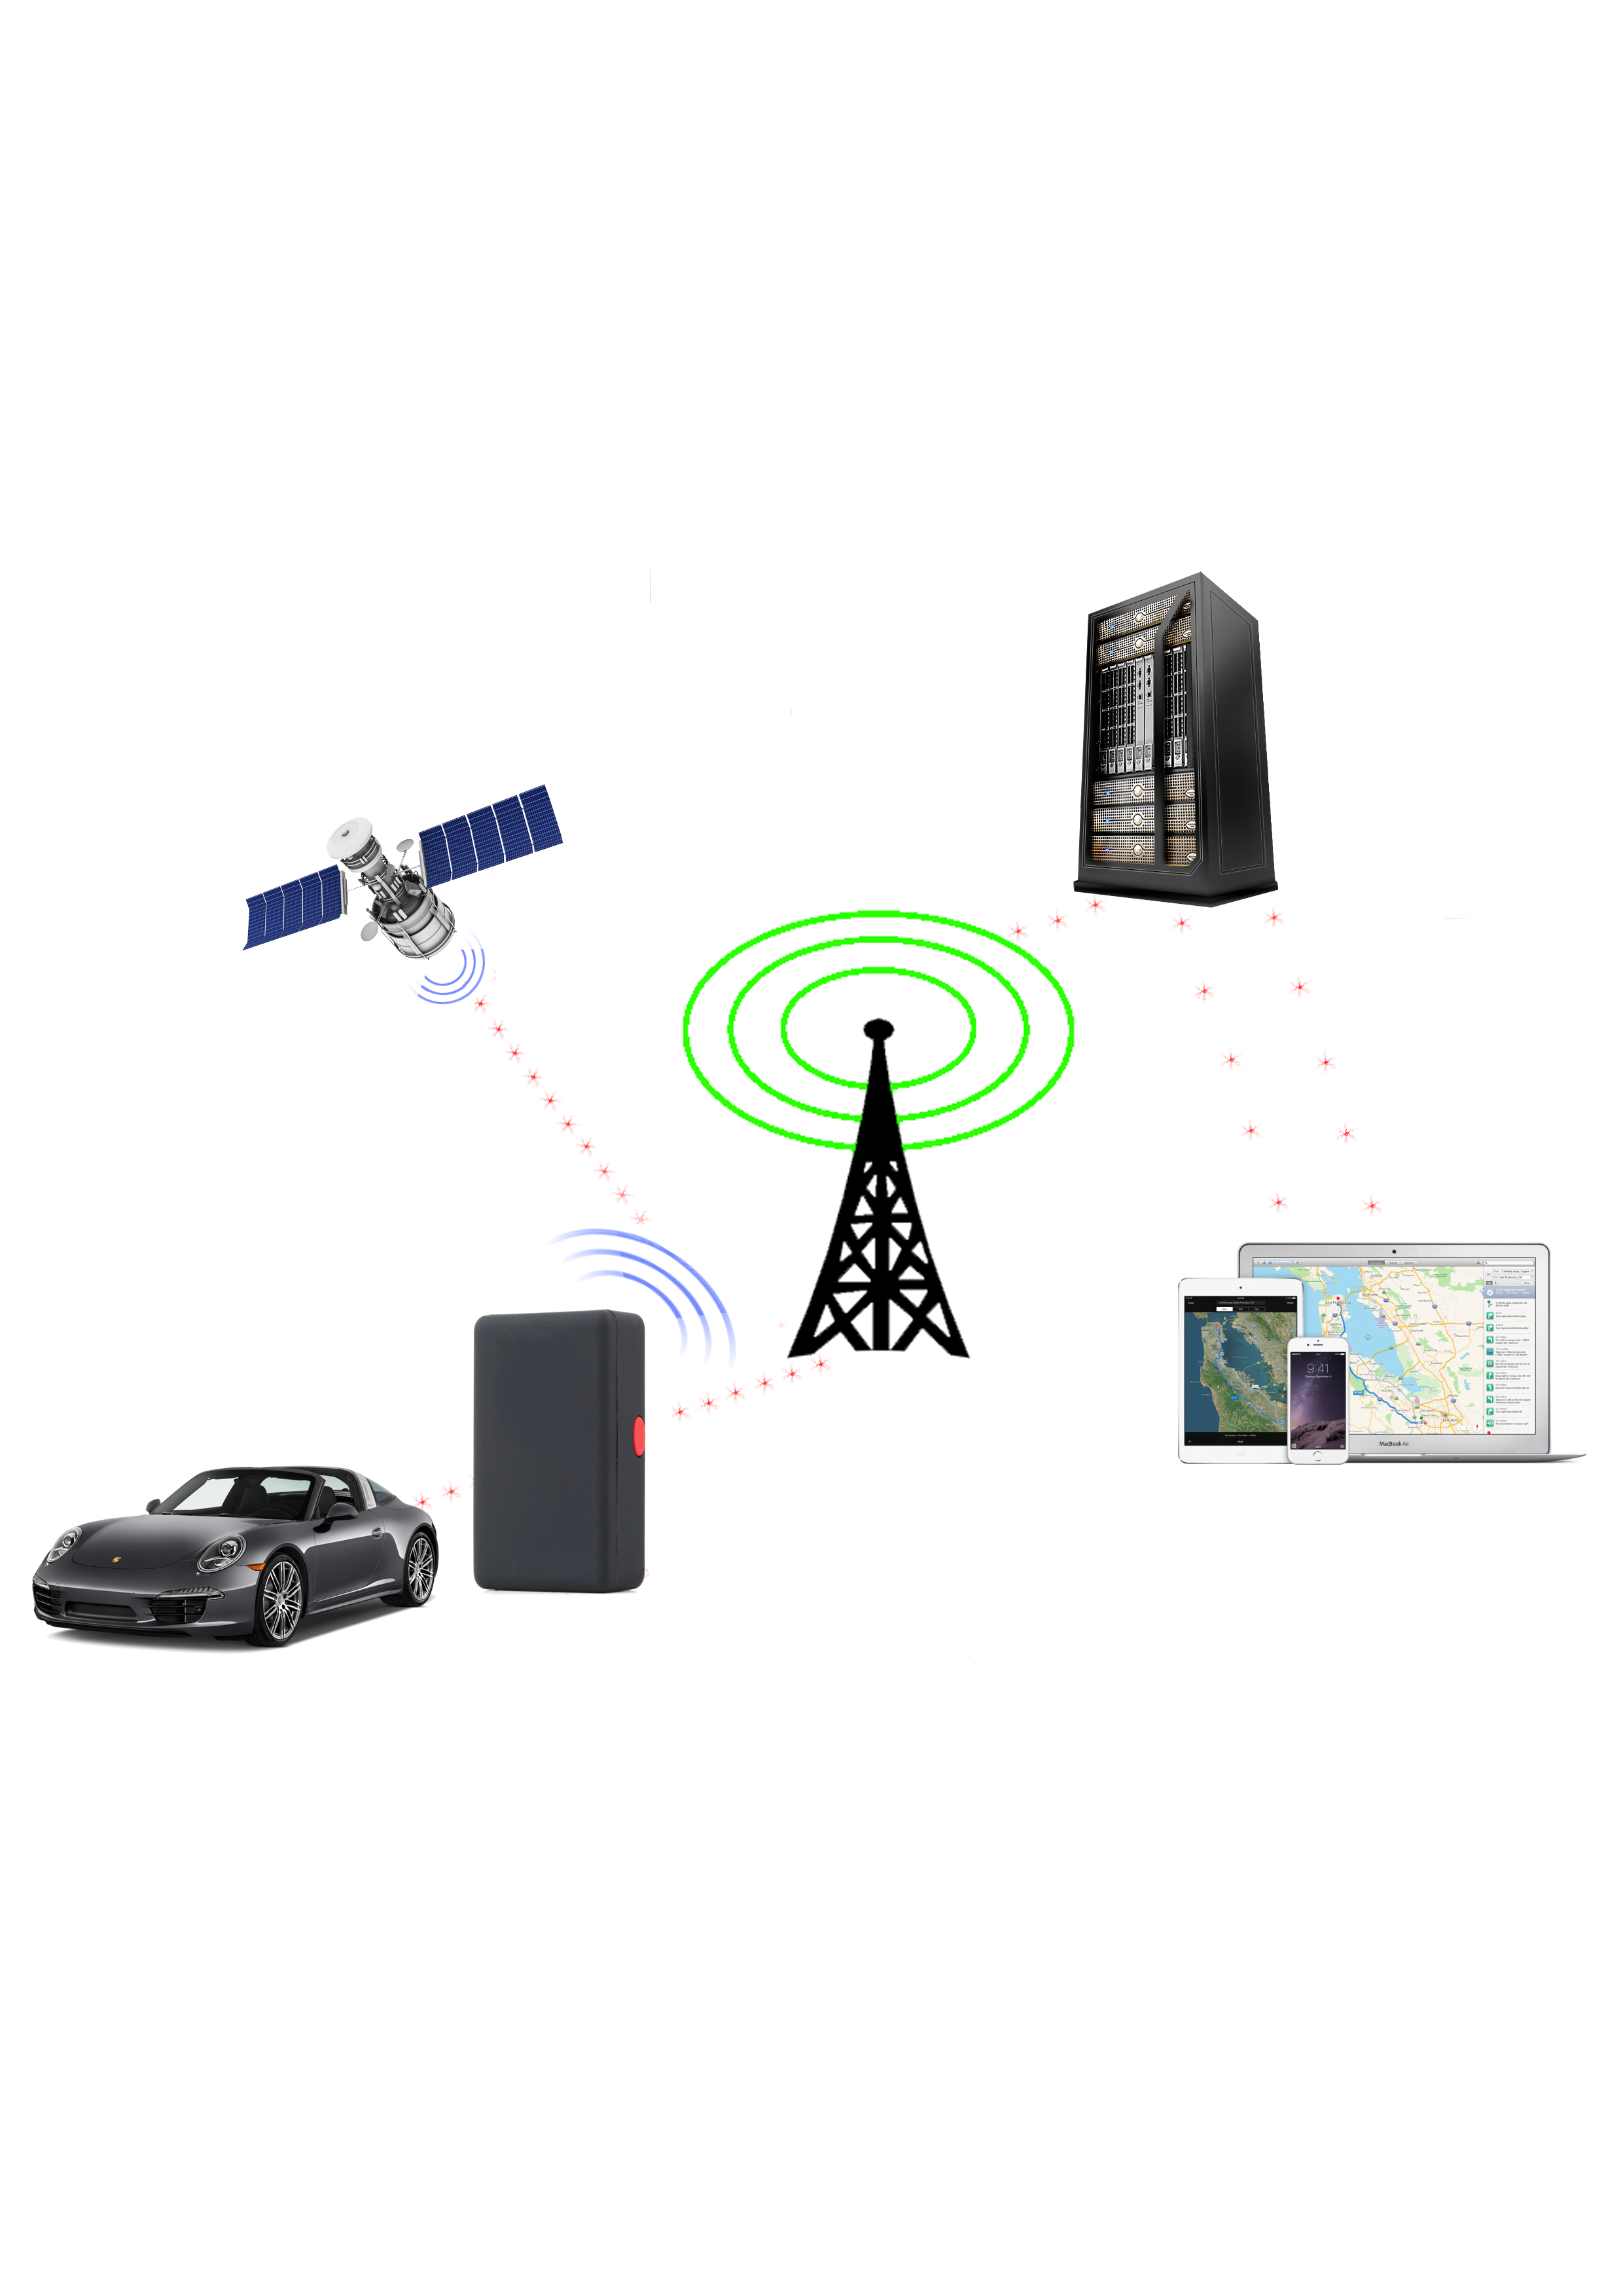
\includegraphics[trim={0 6cm 0 6cm}, clip, scale=.5]{../Vision/Concetto2.png}
\end{frame}

\pagebreak

\section{Documento di Caratteristiche}
\begin{frame}
\frametitle{Architettura}
Il sistema è composto di diverse componenti hardware e software, utili a fornire un funzionamento agevole  e un'ampia interoperabilità. \\
Tra queste possiamo annoverare: 
\begin{itemize}
\item Una centralina dotata di un modulo GSM, periferica GPS e input seriale per l'acquisizione dei contenuti multimediali.  Il modulo integrato deve essere collegato ad un sistema di alimentazione indipendente dalla batteria, in modo da garantire il funzionamento in qualunque occasione (es. rimozione batteria del veicolo).
\item Database Centralizzato per la memorizzazione dei dati.
\item Applicazione Web per la consultazione delle informazioni richieste.
\end{itemize}

Tale configurazione permette di mantenere la massima interoperabilità tra le parti, senza inficiare la semplicità di utilizzo.
\end{frame}

\begin{frame}
\frametitle{Modello Logico}
Lo schema seguente mostra come viene regolato lo scambio di dati tra il modulo di TrackMyCar, il database e l'applicazione web per la gestione dei contenuti.\\

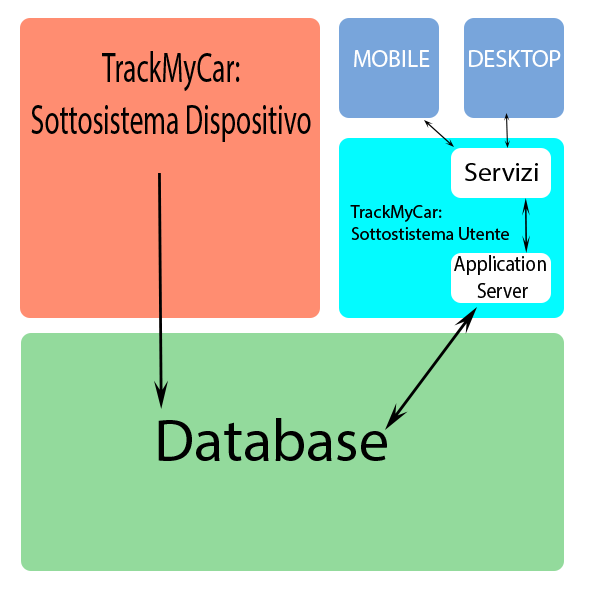
\includegraphics[scale=.3]{../IMG/ModLogico.png}
\end{frame}

\begin{frame}
\frametitle{Modello Fisico}
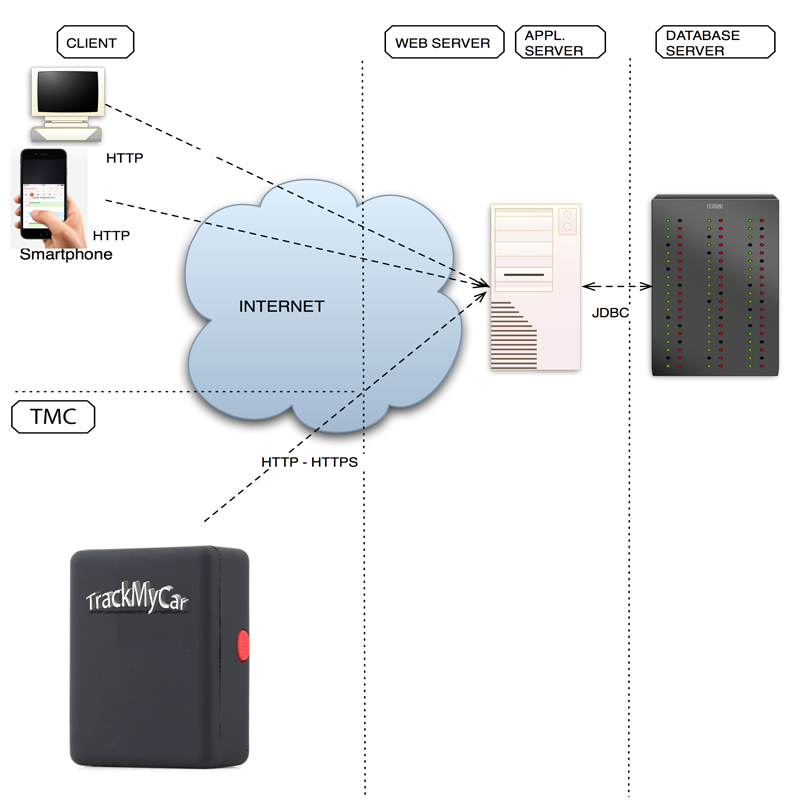
\includegraphics[scale=.3]{../IMG/ModFisico.png}
\end{frame}

\begin{frame}
\frametitle{Tecnologie}
\begin{table}[h]
Gli elementi tecnologici impiegati sono i seguenti:
\begin{center}
\begin{tabular}{ p{3,5cm}  p{5,5cm} }
\rowcolor{Ash}
\hline	
Tipo & Versione \\ \hline
Protocollo & TCP-IP \\ 
Ambiente & Java 2 Enterprise Edition \\ 
Sistema Operativo & Windows, Linux, Mac OS X \\ 
Motore Database & POSTGRESQL 9.4 \\ 
Application Server & Tomcat 7 \\ \hline
\end{tabular}
\end{center}
\end{table}
\end{frame}

\begin{frame}
\frametitle{Requisiti Funzionali}

\begin{center}
\begin{tikzpicture}
\tikzumlset{fill usecase=white!10}

\umlusecase[x=2, y=5, width=5cm]{Gestione Utenti}
\umlusecase[x=2, y=4.2, width=5cm]{Gestione Veicoli}
\umlusecase[x=2, y=3.4, width=5cm]{Associazione Guidatore-Veicolo}
\umlusecase[x=2, y=2.6, width=5cm]{Impostazione Allarmi}


\umlusecase[x=2, y=1.6, width=5cm]{Visualizza posizione}
\umlusecase[x=2, y=0.6, width=5cm]{Controllo Eccesso Velocità}
\umlusecase[x=2, y=-0.2, width=5cm]{Consultazione Storico Furti}
\umlusecase[x=2, y=-1.2, width=5cm]{Live Tracking}

\umlactor[x=-4, y=3, scale=1]{Amministratore}
\umlassoc{Amministratore}{usecase-1}
\umlassoc{Amministratore}{usecase-2}
\umlassoc{Amministratore}{usecase-3}
\umlassoc{Amministratore}{usecase-4}


\umlactor[x=-4, y=-0.4, scale=1]{Regular}
\umlassoc{Regular}{usecase-5}
\umlassoc{Regular}{usecase-6}
\umlassoc{Regular}{usecase-7}
\umlassoc{Regular}{usecase-8}

\umlinherit{Regular}{Amministratore}

\end{tikzpicture}
\end{center}

\end{frame}

\begin{frame}
\frametitle{Requisiti Non Funzionali}
\textbf{Robustezza:} Messaggi e pagine apposite in caso di errore. \\
\textbf{Sicurezza:} Privilegi diversi per gli utenti, protocolli diversi di comunicazione e trasferimento (JDBC, AJP, HTTPS). \\
\textbf{Prestazioni:} Vincoli su tempi di risposta dell'applicazione, a prescindere dalla rete.

\textbf{Interoperabilità}
\begin{itemize}
\item \textbf{Thin Client:} permette, grazie alla tecnologia HTML, di poter accedere al sistema tramite qualunque elaboratore dotato di browser HTML.
\item \textbf{Mobile Client:} è prevista la possibilità di accesso al sistema anche in mobilità.
\item \textbf{Server:} Avendo scelto la tecnologia Java, è possibile cambiare il sistema operativo del server a condizione che questo disponga di una JVM, senza influire sull'applicazione se non per i cambiamenti dei parametri derivanti dalle differenze nei file system.
\end{itemize}
\end{frame}

\begin{frame}
\textbf{Portabilità}
\begin{itemize}
\item \textbf{Thin/Mobile Client:} permette, grazie alla tecnologia HTML, di poter accedere al sistema tramite qualunque dispositivo dotato di browser HTML.
\item \textbf{Server:} Avendo scelto la tecnologia Java, è possibile cambiare il sistema operativo del server a condizione che questo disponga di una JVM, senza modifiche o ricompilazioni.
\end{itemize}
\textbf{Scalabilità}
Essendo il nostro sistema basato su Java Enterprise Edition, architettura altamente scalabile, in caso di numero elevato di utenti sarà possibile servire le richieste tramite una semplice clonazione dell'application server e una configurazione adeguata del load balancing, senza ulteriori interventi sul software.
\pagebreak
\end{frame}

\begin{frame}
\frametitle{Funzioni per l'utente}
Gli attori di questo sistema sono due:
\begin{itemize}
\item Amministratore : Un amministratore gestisce i dati relativi agli utenti, ai gruppi ed alle funzioni ed i permessi ad operare. Può inoltre gestire l'associazione dei veicoli ai rispettivi utilizzatori, gli allarmi e le notifiche via SMS e mail. Tutte le funzioni disponibile per il Regular possono comunque essere svolte dall'amministratore.
\item Regular : Le funzioni di un regular user riguardano la consultazione di informazioni relative al veicolo tracciato, come schematizzato in precedenza.
\end{itemize}

\textbf{Standard}
\begin{itemize}
\item Tecnologia GPS
\item J2EE
\end{itemize}

\textbf{Documentazione:} A supporto dell'applicativo saranno realizzati un Manuale Utente in formato elettronico, consultabile e scaricabile dal sito del prodotto.
\end{frame}
\pagebreak

\section{Documento di Specifiche dei Casi D'Uso}
\begin{frame}
\frametitle{Funzioni Comuni}
\begin{center}
\begin{tikzpicture}
\tikzumlset{fill usecase=white!10}
\umlusecase[x=2, y=1.5, width=5cm]{Login}
\umlusecase[x=2, y=-1.5, width=5cm]{Logout}

\umlactor[x=-2, scale=1.5]{User}
\umlassoc{User}{usecase-9}
\umlassoc{User}{usecase-10}

\end{tikzpicture}
\end{center}
\end{frame}

\begin{frame}
\frametitle{Login}
Coloro che si collegano al sito di TrackMyCar, tramite il loro browser, verranno accolti da una schermata di login in cui inserire le proprie credenziali di accesso. Il sistema ne verifica la correttezza: in caso affermativo si procede alla consultazione della propria area riservata, altrimenti verrà mostrato a video un messaggio di errore.
\begin{center}
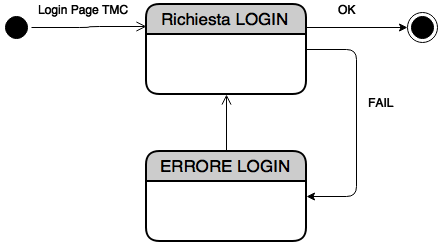
\includegraphics[scale=0.5]{../UseCase/Login.png}
\end{center}
\end{frame}

\begin{frame}
\frametitle{Logout}
L'utente può effettuare il logout da qualunque pagina, a parte le pagine di errore e quelle di login. Premendo sul tasto dedicato, si viene indirizzati nuovamente alla pagina di login del sito.
\begin{center}
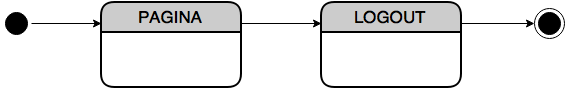
\includegraphics[scale=0.5]{../UseCase/Logout.png}
\end{center}
\end{frame}

\begin{frame}
\frametitle{Funzioni Regular}
\begin{center}
\begin{tikzpicture}
\tikzumlset{fill usecase=white!10}

\umlusecase[x=2, y=-3.5, width=5cm]{Visualizza posizione}
\umlusecase[x=2, y=-5, width=5cm]{Controllo Eccesso Velocità}
\umlusecase[x=2, y=-6.5, width=5cm]{Consultazione Storico Furti}
\umlusecase[x=2, y=-8, width=5cm]{Live Tracking}

\umlactor[x=-4, y=-5, scale=1]{Regular}
\umlassoc{Regular}{usecase-11}
\umlassoc{Regular}{usecase-12}
\umlassoc{Regular}{usecase-13}
\umlassoc{Regular}{usecase-14}
\end{tikzpicture}
\end{center}
\end{frame}

\begin{frame}{Visualizza Posizione}
Accedendo al sito di TrackMyCar si possono consultare numerose informazioni riguardo il proprio veicolo, previo login. La pagina che viene restituita contiene una serie di operazioni svolgibili, di competenza dell'utente con privilegi non elevati. Selezionando la voce ``Posizione Veicoli'' si può verificare l'esatta ubicazione dei propri mezzi all'istante desiderato. Tale informazione viene segnalata su una mappa tramite un indicatore di posizione. 

In ogni momento si verifica se l'utente ha i privilegi necessari per accedere ad una determinata funzione, altrimenti viene indirizzato alla pagina di errore. Successivamente viene inviato alla propria home oppure alla pagina di login, secondo i casi.

\begin{center}
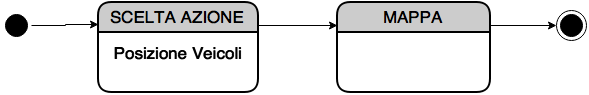
\includegraphics[scale=0.3]{../UseCase/Posizione.png}
\end{center}
\end{frame}

\begin{frame}
\frametitle{Controllo Eccesso di Velocità}
Scegliendo la funzione associata è possibile consultare gli eventuali allarmi provocati dai veicoli a cui l'utente è legato. Nel caso non fosse associato alcun veicolo all'utente, tale evento verrà segnalato tramite un messaggio. 

\begin{center}
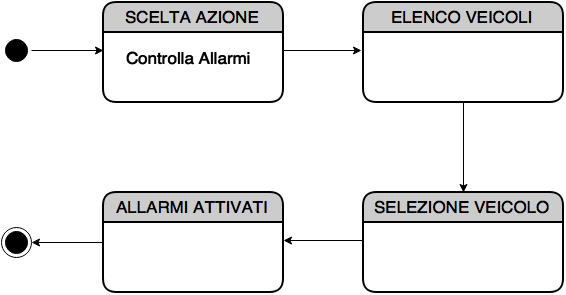
\includegraphics[scale=0.3]{../UseCase/Allarmi.png}
\end{center}
\end{frame}

\begin{frame}
\frametitle{Consultazione Storico Furti}
Funzione che, come da titolo, permette di tenere traccia degli eventuali furti ai danni dei veicoli associati all'utente. Dalla lista puntata, selezionando un furto, è possibile visualizzare a schermo la mappa del percorso effettuato durante la fuga del ladro. Nel caso non fosse associato alcun veicolo all'utente, tale evento verrà segnalato tramite un messaggio.

\begin{center}
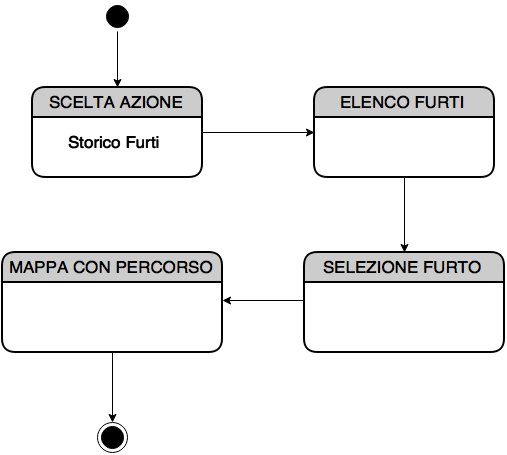
\includegraphics[scale=0.3]{../UseCase/Storico.png}
\end{center}
\end{frame}

\begin{frame}
\frametitle{Live Tracking}
Selezionando la voce associata è possibile visualizzare tramite il proprio browser (in tempo reale) il percorso del veicolo scelto. All'interno della stessa pagina è possibile riprodurre in streaming il video del ladro direttamente dall'abitacolo. Nel caso l'utente non disponga di veicoli o non sia stato derubato, l'applicazione fornirà notifica a video.

\begin{center}
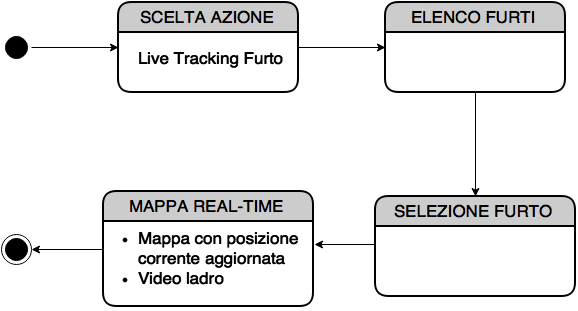
\includegraphics[scale=0.3]{../UseCase/Tracking.png}
\end{center}
\end{frame}

\begin{frame}
\frametitle{Funzioni Amministratore}
\begin{center}
\begin{tikzpicture}
\tikzumlset{fill usecase=white!10}

\umlusecase[x=2, y=4, width=5cm]{Gestione Utenti}
\umlusecase[x=2, y=2.5, width=5cm]{Gestione Veicoli}
\umlusecase[x=2, y=1, width=5cm]{Associazione Guidatore-Veicolo}
\umlusecase[x=2, y=-0.5, width=5cm]{Impostazione Allarmi}


\umlactor[x=-4, y=2, scale=1]{Amministratore}
\umlassoc{Amministratore}{usecase-15}
\umlassoc{Amministratore}{usecase-16}
\umlassoc{Amministratore}{usecase-17}
\umlassoc{Amministratore}{usecase-18}


\end{tikzpicture}
\end{center}
\end{frame}

\begin{frame}
\frametitle{Gestione Utenti}
Attraverso la scelta di questa funzione, l'amministratore può decidere di operare sugli utenti che sfruttano l'applicazione. Le azioni disponibili permettono di aggiungere una nuova utenza, modificarne una esistente oppure eliminarla. Le ultime due funzioni presuppongono la scelta di un profilo da una lista, limitando così la possibilità di errori o incomprensioni per l'utilizzatore finale. La presenza di un amministratore è obbligatoria e non è possibile eliminarlo, in caso sia l'ultimo utente rimasto.
\end{frame}

\begin{frame}
\begin{center}
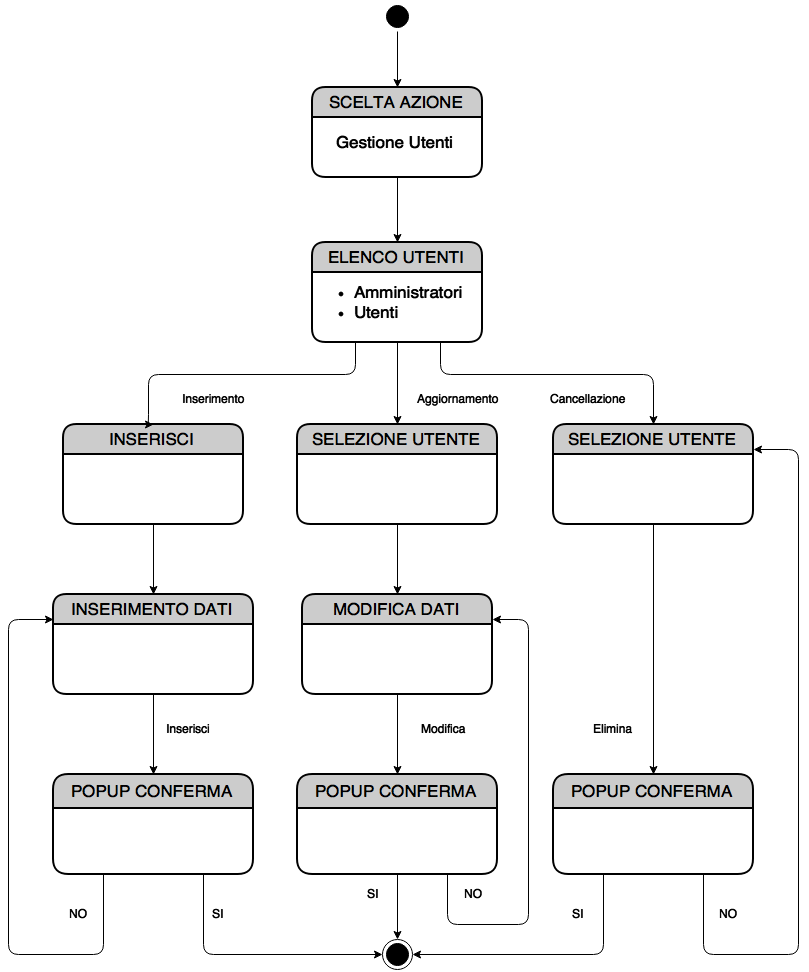
\includegraphics[scale=0.2]{../UseCase/Utenti.png}
\end{center}
\end{frame}

\begin{frame}
\frametitle{Gestione Veicoli}
La selezione di questa funzione permette all'utente di aggiungere o modificare/eliminare un veicolo all'interno della lista. L'elenco dei veicoli e i pulsanti sottostanti permettono di guidare l'utente nella scelta delle operazioni da compiere. Nel caso non siano presenti veicoli, l'utente verrà immediatamente informato da un messaggio a video.
\end{frame}

\begin{frame}

\begin{center}
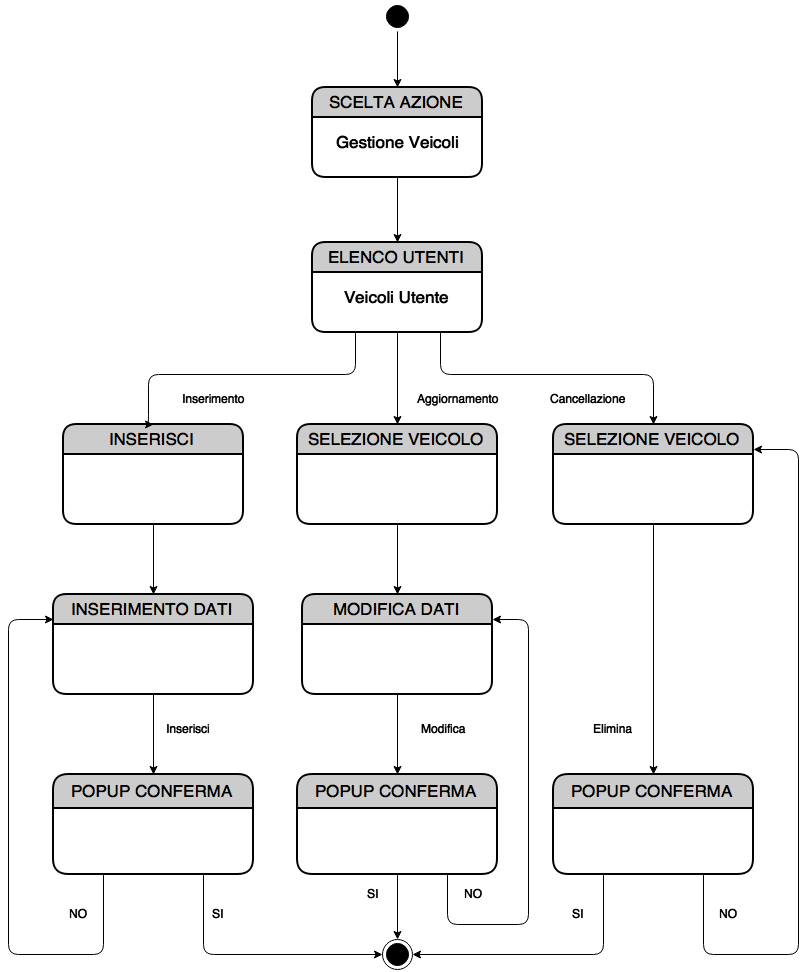
\includegraphics[scale=0.2]{../UseCase/Veicoli.png}
\end{center}
\end{frame}

\begin{frame}
\frametitle{Associazione Guidatore-Veicolo}
La pagina che viene mostrata selezionando la suddetta funzione permette di associare utenti e veicoli presenti nella base di dati. Nel caso non vi siano veicoli, l'utente verrà messo a conoscenza di ciò tramite un messaggio. Non è possibile che non siano presenti utenti da associare per quanto detto in precedenza (vedere Gestione Utenti).
\end{frame}

\begin{frame}
\begin{center}
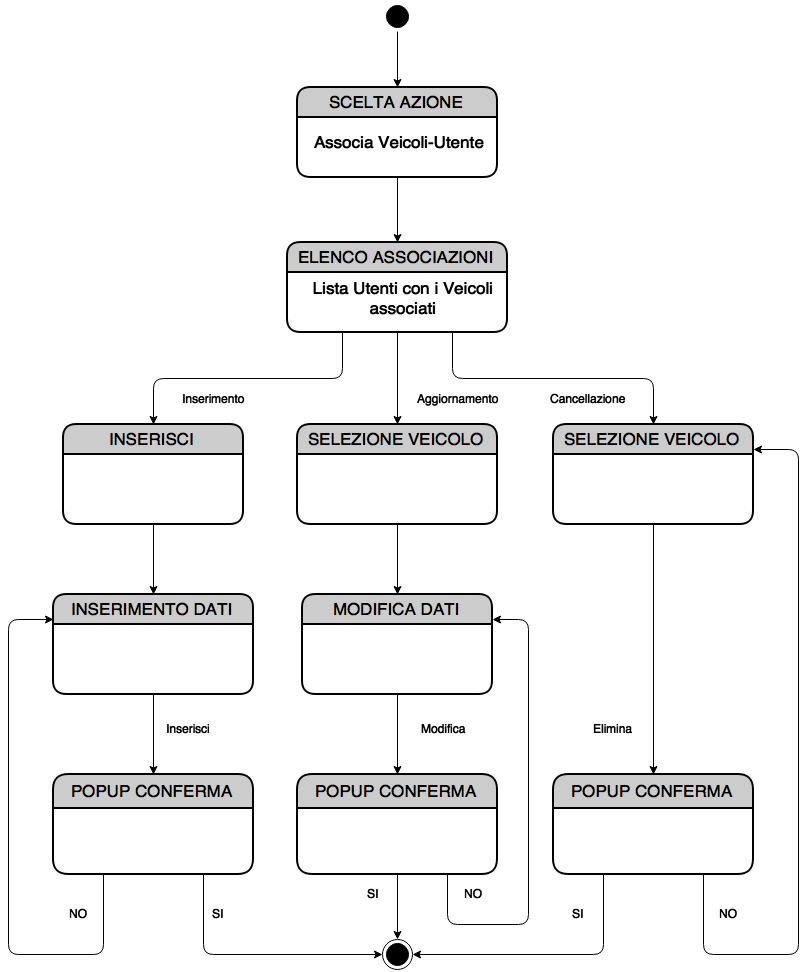
\includegraphics[scale=0.2]{../UseCase/Associa.png}
\end{center}
\end{frame}



\begin{frame}
\frametitle{Impostazione Allarmi}
Scegliendo ``Imposta limite'' dalla pagina del profilo di amministratore, si viene diretti nella pagina di impostazione dei limiti a cui far scattare gli allarmi per eccesso di velocità. Tale funzione può essere espletata scegliendo un veicolo dalla lista e premendo su uno dei due tasti sottostanti la lista. Scegliendo la modifica, il limite verrà reimpostato (di default è 130 Km/h, impostato automaticamente in fase di inserimento di un nuovo veicolo), altrimenti questo può essere azzerato, eliminando le future notifiche agli utenti associati ai veicoli interessati.
\end{frame}

\begin{frame}

\begin{center}
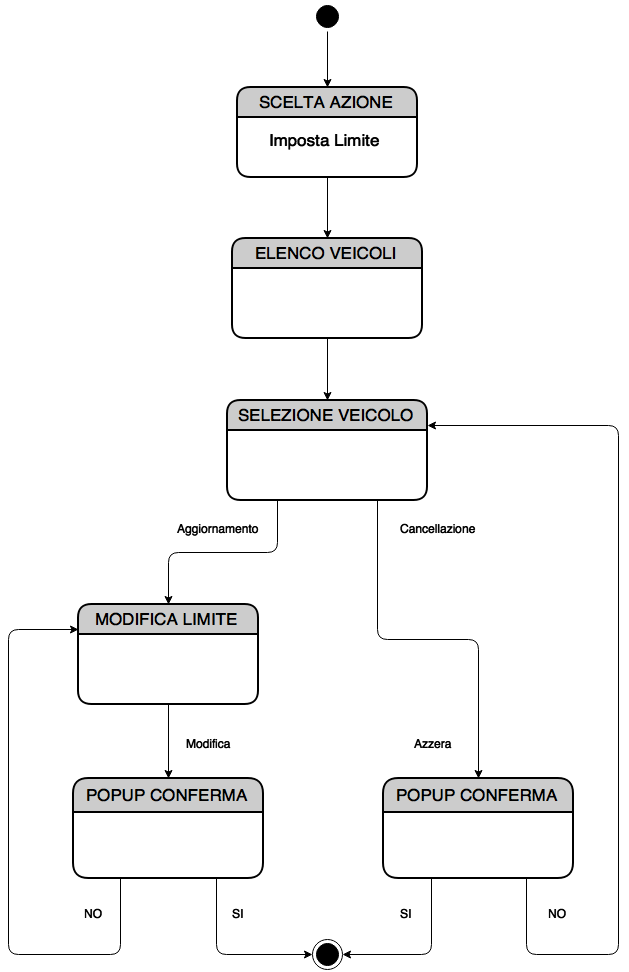
\includegraphics[scale=0.2]{../UseCase/Limite.png}
\end{center}
\end{frame}


\pagebreak

\section{WBS}
\begin{frame}
\frametitle{WBS}
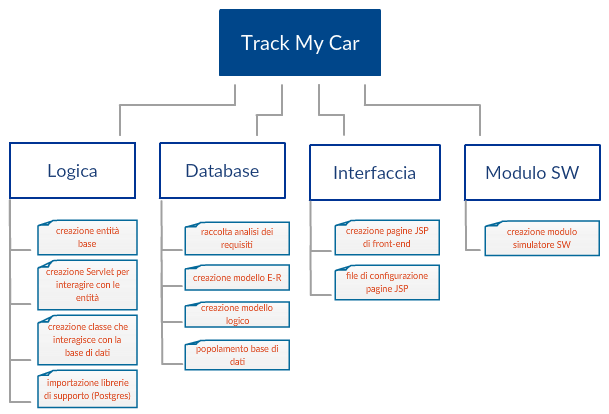
\includegraphics[scale=.5]{wbs.png}
\end{frame}

\pagebreak

\section{OBS}
\begin{frame}
\frametitle{OBS}
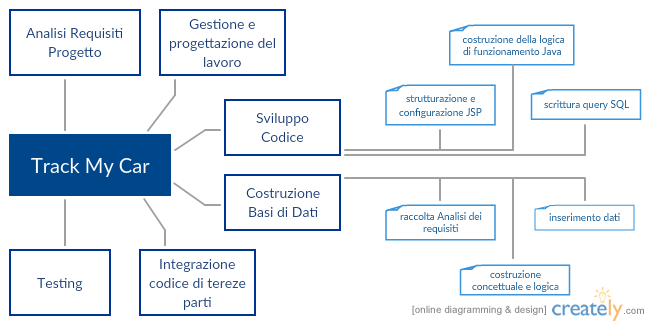
\includegraphics[scale=.5]{obs.png}
\end{frame}


\pagebreak

\section{Documento di Project Plan}
\begin{frame}
\frametitle{Organizzazione di Progetto}
Nel progetto verranno affrontate le seguenti attività:
\begin{itemize}
\item Documentazione di Progetto
\begin{itemize}
\item Analisi dei Requisiti
\item Gestione Tecnica del Progetto
\end{itemize}
\item Database
\begin{itemize}
\item Progettazione 
\item Popolamento
\end{itemize}
\item Applicazione Web
\begin{itemize}
\item Logica applicativa
\item Interfaccia utente
\end{itemize}
\item Realizzazione modulo HW e installazione
\item Test
\end{itemize}
\end{frame}

\pagebreak

\section{RAM / RACI}
\begin{frame}
\frametitle{Matrice di responsabilità}
\begin{table}[ht]
\begin{center}
\begin{tabular}{l | l | l | l}
\rowcolor{Ash}
\hline
\multicolumn{1}{ c |}{\multirow{2}{*}{Attività}}      & \multicolumn{3}{c}{Ruoli} \\ \cline{2-4}
\rowcolor{Ash}
  							    & Mansoldo & Dal Monte & Vicentini \\ \hline
 Documentazione di progetto & R & C & A \\ \hline
 Progettazione Database	    & A & R & C \\ \hline
 Popolamento Database	    & I  & R & A \\ \hline
 Logica Applicativa webapp   & A & C & R \\ \hline
 Interfaccia Utente			    & C & A & R \\ \hline
 Realizzazione Modulo HW   & I  & R &  A \\ \hline
 Manuale Utente			    & R & A & C \\ \hline
 Test						    & R & R & A \\ 
\hline
\end{tabular}
\end{center}
\end{table}


\begin{table}[ht]
\begin{center}
\begin{tabular}{c | c}
\hline
R & Responsible \\
A & Accountable \\
C & Consulted \\
I  & Informed \\ \hline
\end{tabular}
\end{center}
\end{table}
\end{frame}

\pagebreak

\begin{frame}
\frametitle{Reticolo delle precedenze}
\footnotesize{
\begin{table}[ht]
\begin{center}
\begin{tabular}{c | c | c | c | c}
\rowcolor{Ash}
\hline
Milestone & Codice    					     & Durata & Predecessore & Successore \\ \hline
Inizio        & 	       		    					     &  		 &  				  &  \\ \hline
& & &  & PrDB \\
& Docs  & 7 & Inizio & LogA \\
& & &  & IntU \\
& & &  & ReHW \\ \hline
& PrDB   	    & 3 & Docs & PoDB \\ \hline
& PoDB    	    & 1 & PrDB & Test \\ \hline
& LogA        & 10 & Docs & Test \\ \hline
& IntU       			    & 8 & Docs & ManU \\ 
& & & &  Test \\ \hline
& ReHW   &  5 & Docs & Test \\ \hline
& ManU    &  1 & IntU & Fine \\ \hline
& & &  PoDB & \\
& Test       						    & 3  & LogA & Fine \\ 
& & &  IntU & \\
& & &  ReHW & \\ \hline
Fine & 						    &  &  &  \\\hline
\end{tabular}
\end{center}
\end{table}}
\end{frame}

\pagebreak

\section{Reticolo di Progetto / CPM}
\begin{frame}
\frametitle{CPM}
\begin{figure}[htbp]
\centering
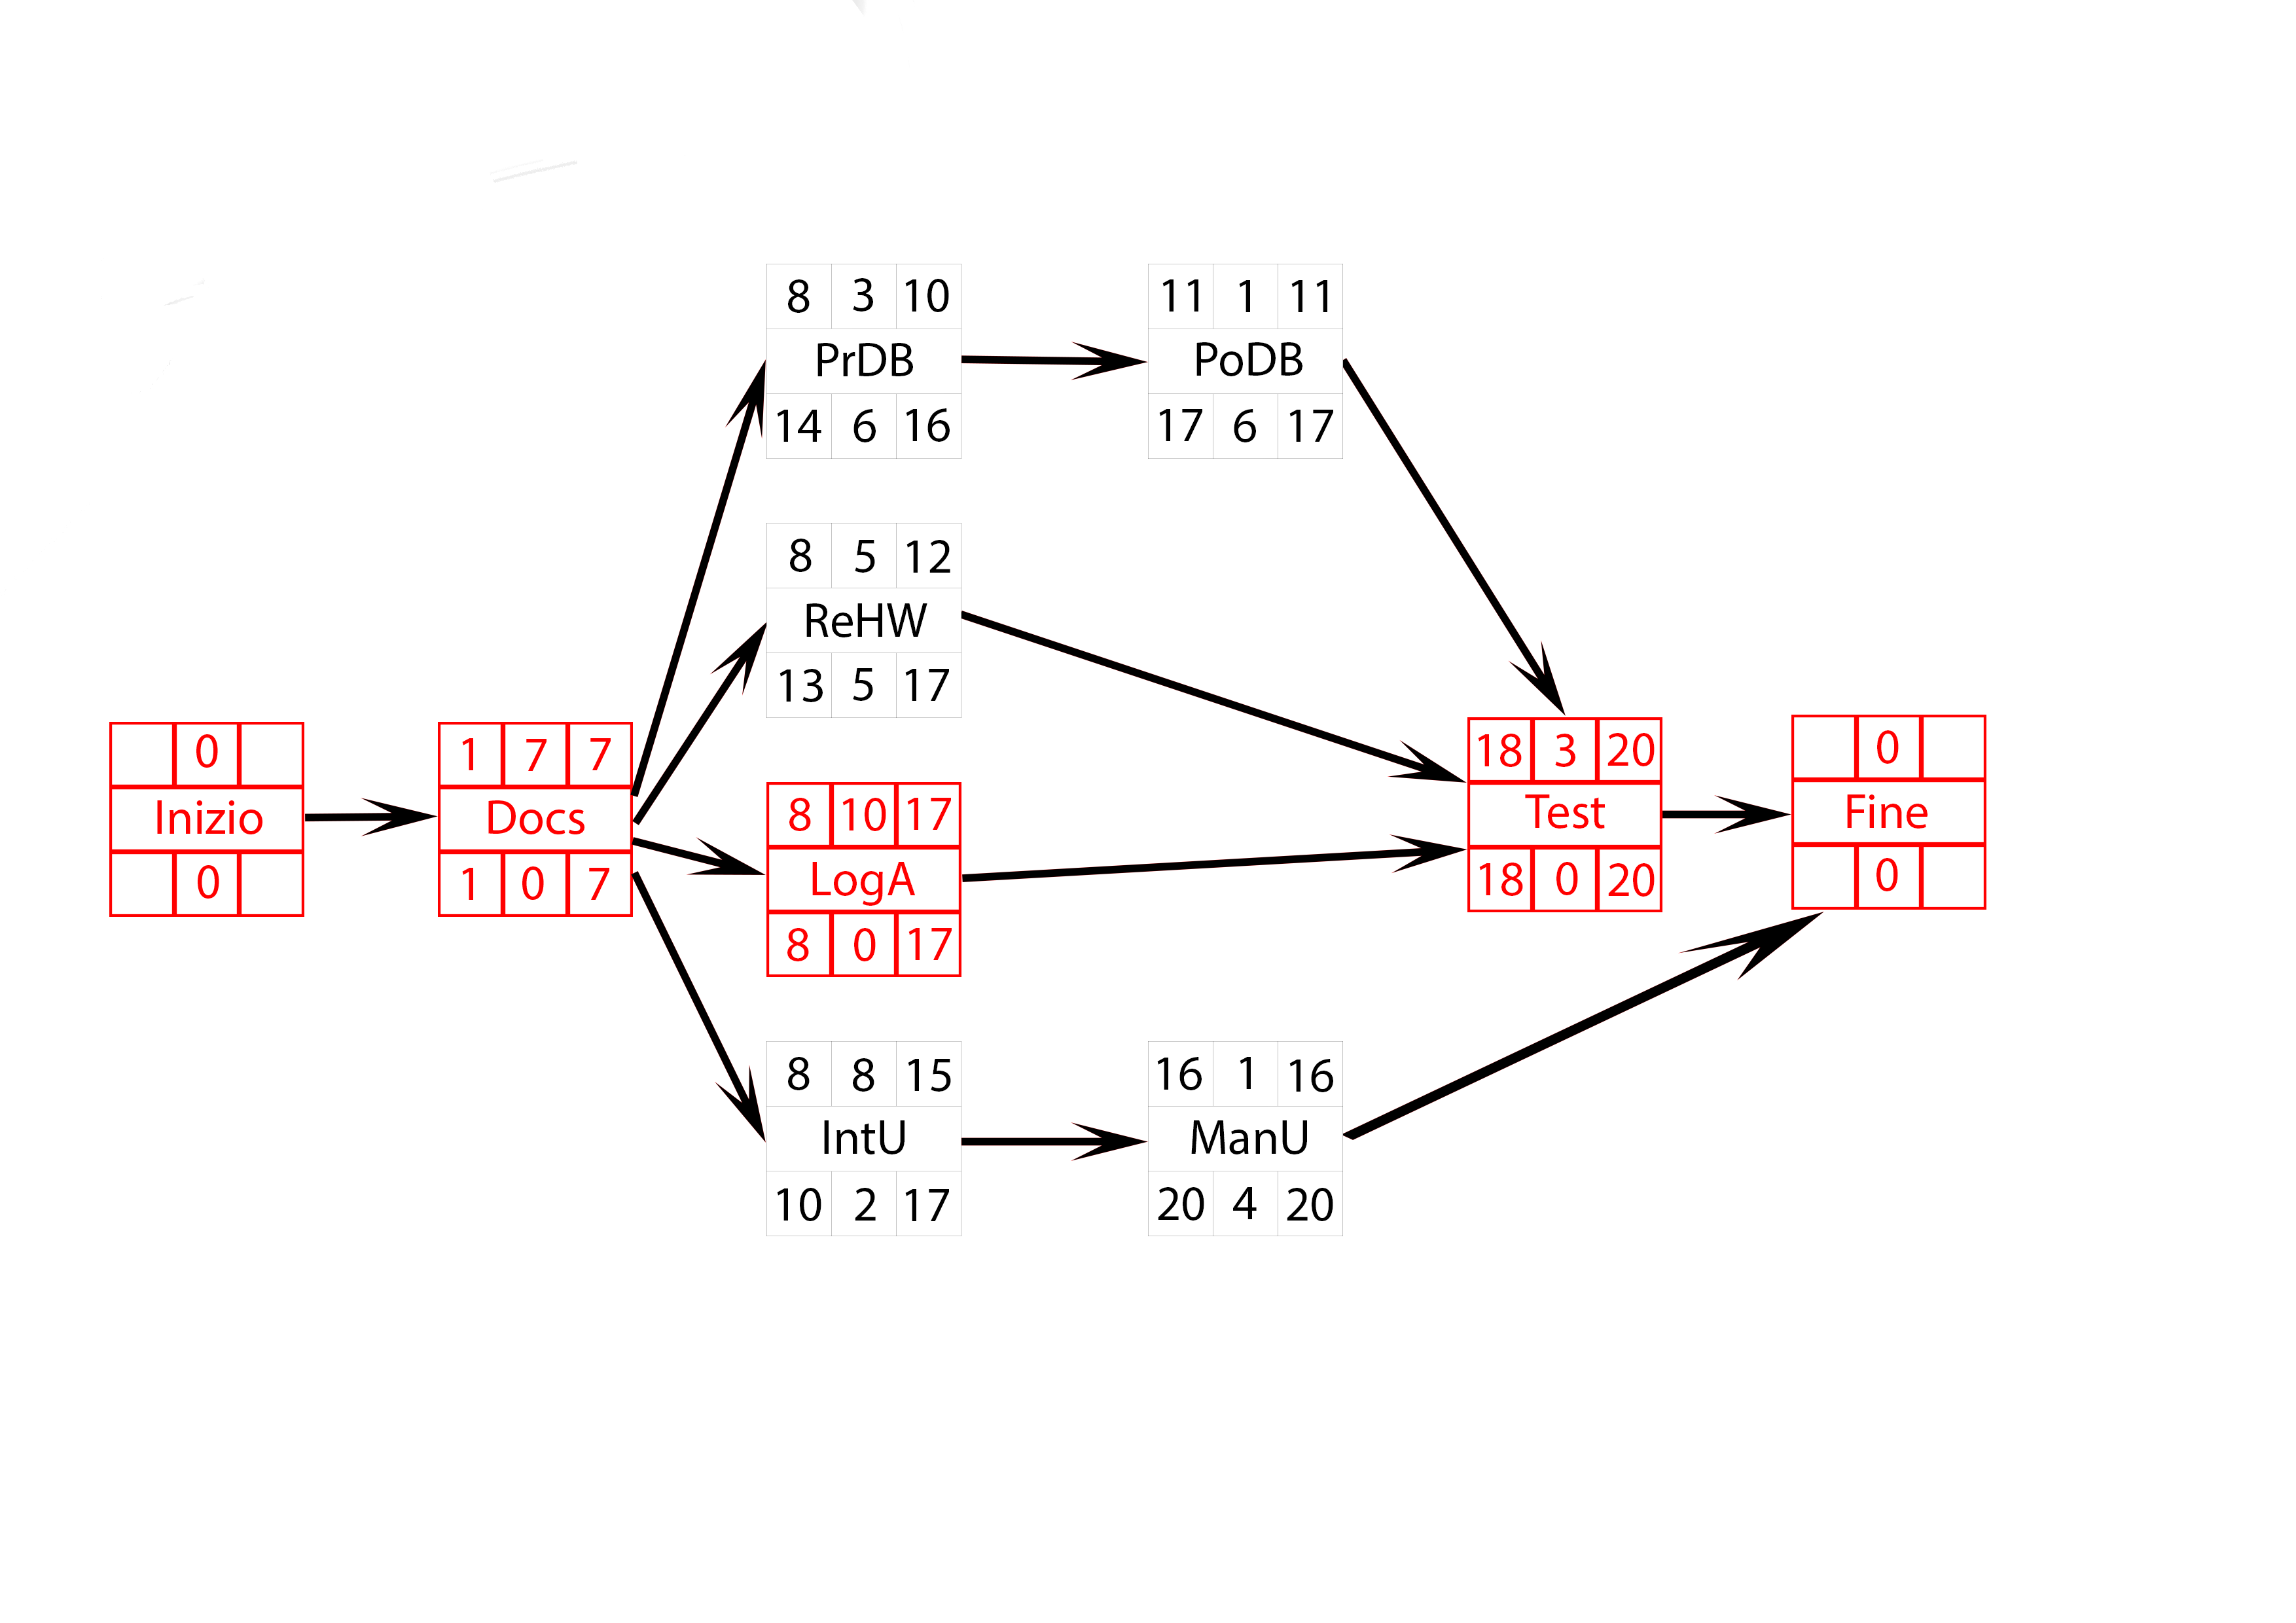
\includegraphics[trim={1cm 4.5cm 3.5cm 2.5cm}, clip, scale=0.3]{../ProjectPlan/CPM.png}
\end{figure}
\end{frame}

\begin{frame}
\frametitle{Deliverables}
Il completamento delle attività sovrastanti produrrà i seguenti deliverables:
\begin{itemize}
\item Database su cui verranno salvati i dati ricevuti dal modulo di Track~My~Car
\item La centralina Hardware da installare fisicamente sul veicolo
\item Webapp di gestione del modulo (JSP)
\item Documentazione a supporto (Manuale Utente)
\end{itemize}
\end{frame}

\pagebreak

\section{Cronoprogramma}
\begin{frame}
\frametitle{Cronoprogramma}
\begin{figure}[htbp]
\centering
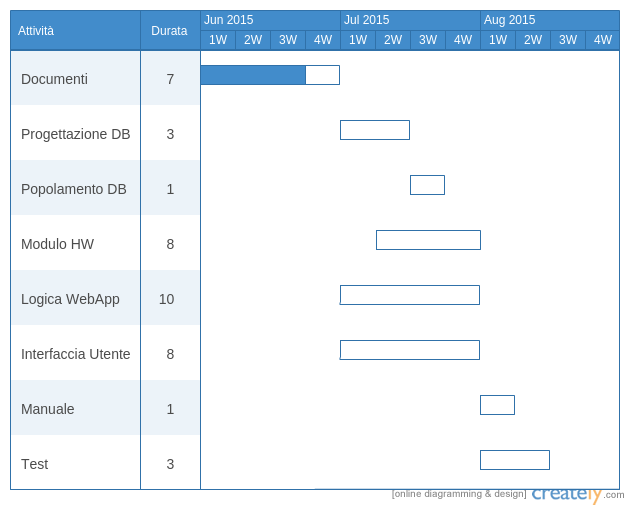
\includegraphics[trim={0 0.66cm 0 0}, clip, scale=0.4]{../ProjectPlan/gantt.png}
\end{figure}
\end{frame}

\begin{frame}
\frametitle{Calendario di Progetto}
\begin{table}[ht]
\begin{center}
\begin{tabular}{l | l | l}
\rowcolor{Ash}
\hline
Data Inizio        & Data Fine	      &  	Oggetto	     \\ \hline
01/06/2015 & 30/06/2015 & Documentazione di progetto  \\ \hline
01/07/2015 & 10/07/2015 & Progettazione Database	     \\ \hline
11/07/2015 & 12/07/2015 & Popolamento Database	     \\ \hline
11/07/2015 & 20/07/2015 & Realizzazione Modulo HW    \\ \hline
10/07/2015 & 10/08/2015 & Logica Applicativa webapp    \\ \hline
10/07/2015 & 10/08/2015 & Interfaccia Utente			     \\ \hline
11/08/2015 & 12/08/2015 & Manuale Utente			     \\ \hline
19/08/2015 & 10/09/2015 & Test						     \\ \hline
\end{tabular}
\end{center}
\end{table}
\end{frame}

\pagebreak

\section{Infrastruttura di Progetto}
\begin{frame}
\frametitle{Infrastruttura di Progetto}
\begin{itemize}
	\item Workspace Sorgenti Webapp
	\begin{itemize}
		\item Package su Macchina di Sviluppo (directory locale)
		\item Repository GitHub
	\end{itemize}
	\item Workspace Documentazione
	\begin{itemize}
		\item Package su Macchina di Sviluppo (directory locale)
		\item Sincronizzazione online tramite file hosting service (Copy)
		\item Repository GitHub
	\end{itemize}
	\item Canale di Comunicazione Interno al Team (Slack)
	\item Ambienti di Rilascio
	\begin{itemize}
		\item Test su PC di sviluppo (Linux Mint, basato su Ubuntu)
		\item Collaudo su PC dell'università (Ubuntu 14.04 LTS)
		\item Rilascio su Macchina del Cliente (dotata di Tomcat e Browser Web)
	\end{itemize}
\end{itemize}
\end{frame}



\pagebreak

\section{Documento di Risk List}
\begin{frame}
\frametitle{Lista dei Maggiori Rischi}
\footnotesize{
\begin{table}[h]
\begin{center}
\begin{tabular}{ p{4cm} p{2cm} p{3cm} } 
\rowcolor{Ash}	
\hline	
Rischio & Gravità & Descrizione  \\ \hline
Consegna progetto oltre il 14 Settembre & Molto Dannoso & Rilascio software oltre la data di scadenza. \\ 
Integrazione Componenti & Molto Dannoso & Fallimento nell'integrazione delle componenti e non raggiungimento degli obbiettivi  \\ 
Mancanza di personale & Dannoso & Assenza di personale per svolgere compiti \\ 
Conoscenza Tecnologie & Medio & Conoscere il funzionamento interno delle tecnologie utilizzate \\ 
Implementazione Multilinguismo & Bassa & Fornire un'interfaccia utente multilingua  \\ \hline
\end{tabular}
\end{center}
\end{table}}
\end{frame}

\pagebreak

\section{Design}
\begin{frame}
\frametitle{Politiche di Riuso}
\small{
La politica del riuso che abbiamo adottato riguarda gran parte del progetto. La struttura della webapp è stata adattata da progetti svolti in precedenza dal team, variando il minimo indispensabile per la riuscita dello stesso.

L'impiego di Servlet unite alla tecnologia JSP ci ha permesso di rendere altamente modulare il nostro codice, favorendo l'aggiunta di nuove funzionalità in modo semplice e rapido, rispetto all'eventualità di implementare ulteriori classi (tecnica piuttosto dispersiva).

Altro elemento fondamentale nel riuso è stato l'impiego di un software COTS, basti pensare al DBMS Postgresql che si interfaccia con la nostra applicazione, fornendo e immagazzinando dati attraverso il driver(intercambiabile con altri DBMS senza inficiare il funzionamento dell'applicazione, es MySQL).

Infine la metodologia di sviluppo di software impiegata può essere accostata facilmente ad una logica di tipo Model-View-Controller, framework molto utile nella progettazione di interfacce grafiche e logiche applicative (Java-JSP).}
\end{frame}

\pagebreak

\section{Diagramma dei Package}
\begin{frame}
\frametitle{Diagramma dei Package}
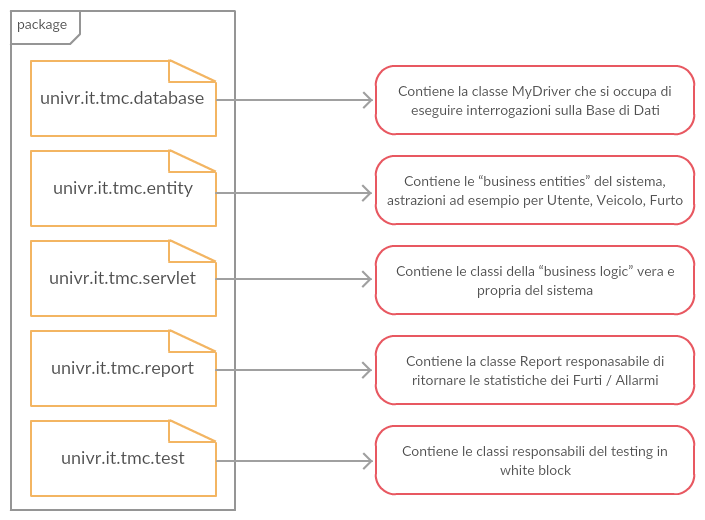
\includegraphics[scale=.4]{packageDiagram.png}
\end{frame}

\pagebreak

\section{Diagramma delle Classi}
\begin{frame}
\frametitle{Diagramma delle Classi}
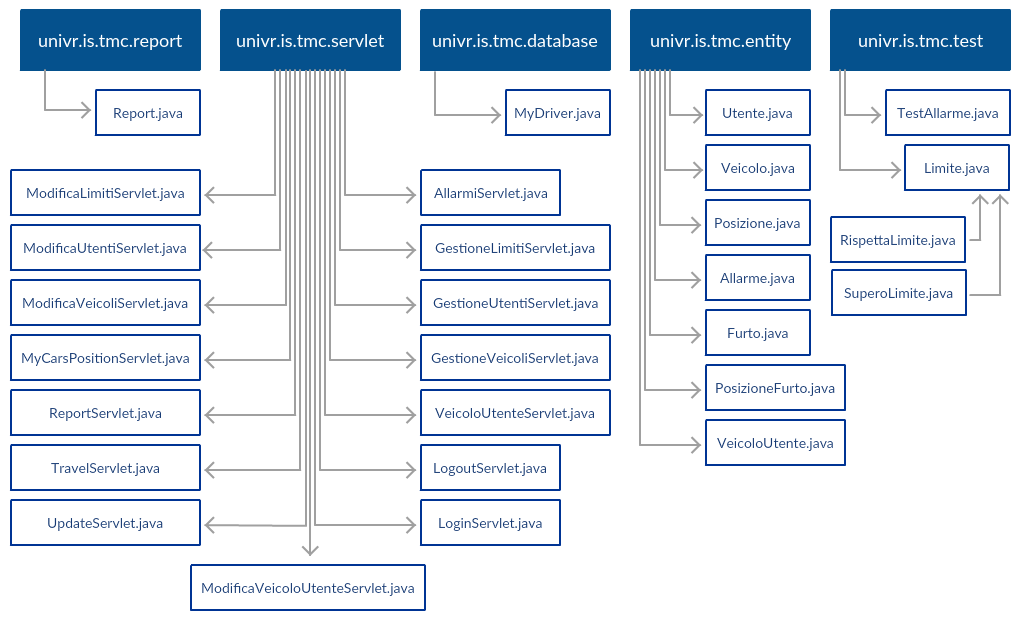
\includegraphics[scale=.3]{classDiagram.png}
\end{frame}

\pagebreak

\section{Diagramma delle Sequenze}
\begin{frame}
\frametitle{Login diagram state}
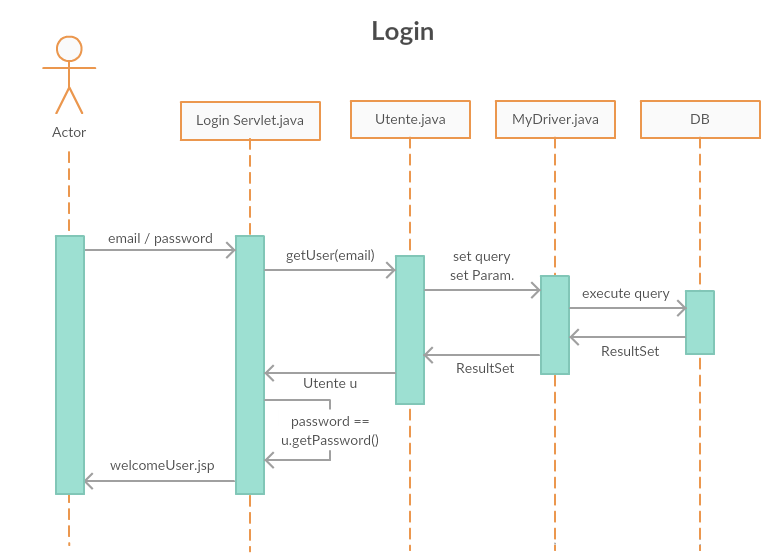
\includegraphics[scale=0.4]{LoginSeq.png}
\end{frame}

\begin{frame}{Admin diagram state}
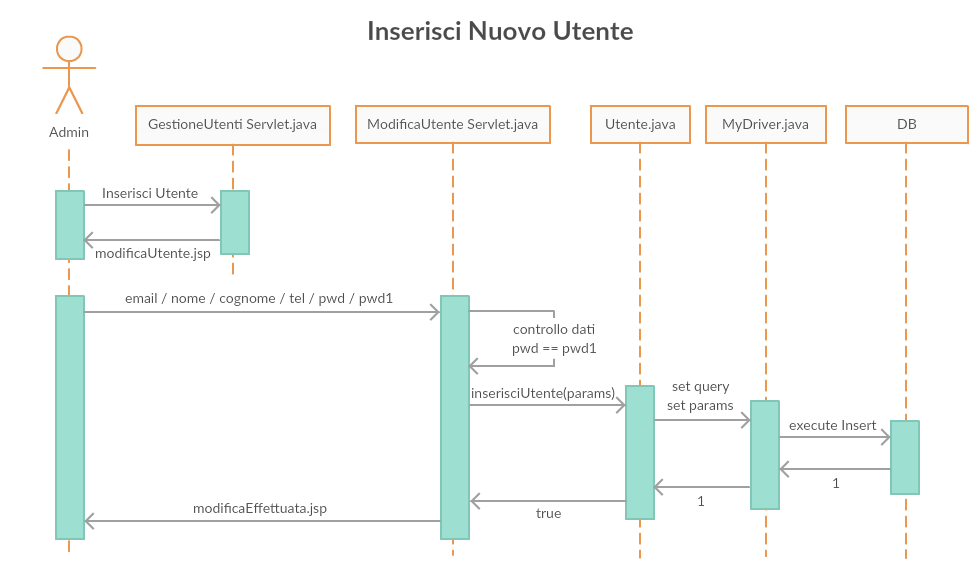
\includegraphics[scale=0.32]{AdminSeq.png}
\end{frame}

\begin{frame}
\frametitle{Regular diagram state}
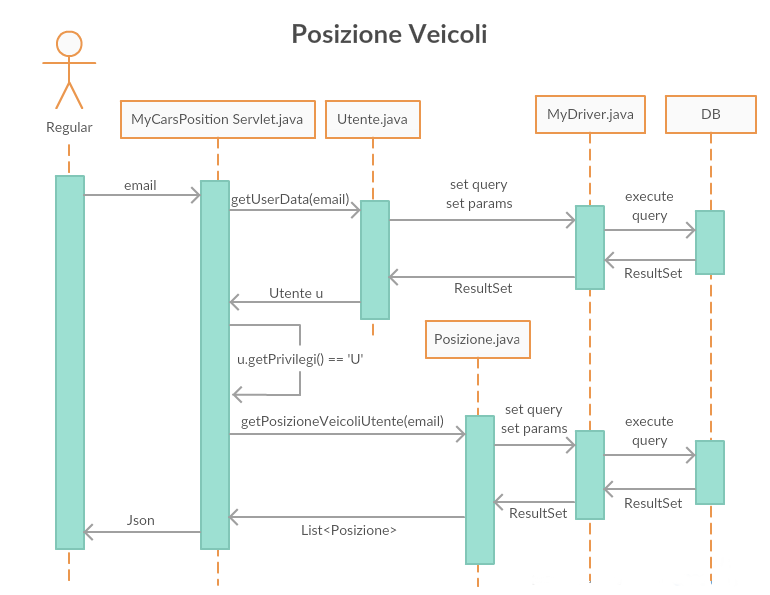
\includegraphics[scale=0.38]{RegularSeq.png}
\end{frame}

\pagebreak

\section{Design Pattern}
\begin{frame}
\frametitle{Design Pattern}
Essendo il progetto piccolo, non si è reso necessario l'utilizzo di particolari design pattern. Questo però non ha impedito al gruppo di immaginare scenari in cui includere alcuni di essi. 

Possibile implementazione Factory
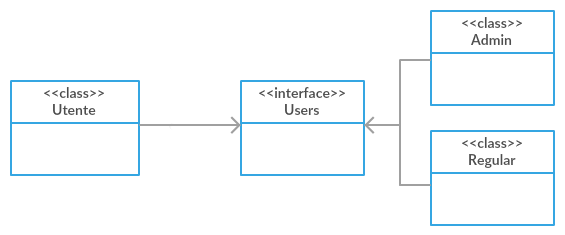
\includegraphics[scale=.5]{DesignPattern.png}
\end{frame}

\begin{frame}
Nel nostro progetto viene spesso 
Nel nostro progetto viene spesso richiesto di ritornare dei risultati diversi in base all'utente corrente.\\
Funzioni Regular:\\
> Posizione Corrente: ritorna posizione dei veicoli associati.\\
> Live Tracking: ritorna lista furti attivi dei veicoli associati.\\
> Allarmi Veicolo: ritorna lista veicoli associati.\\
> Storico Furti: ritorna lista furti dei veicoli associati.\\
Tutte queste funzioni dell'utente Regular, sono più flessibili in caso l'utente corrente fosse un Amministratore. Infatti in tal caso vengono visualizzate tutti i Veicoli/Furti anche se non direttamente associati a lui.
L'implementazione lato back-end di questo, con l'utilizzo di una Abstract Factory sarebbe piu agevole:\\
\small{
String email = request.getSession().getAttribute("currUserEmail");\\
Utente u = Utente.getUserData(email);\\
if( u.instanceOf(Admin) ) return lista A;\\
else if( u.instanceOf(Reguler) ) return lista B;}
\end{frame}

\pagebreak

\section{Principi SOLID}
\begin{frame}
\frametitle{Principi SOLID Utilizzati}
\begin{itemize}
\item Single Responsibility Principle : un cambiamento su una classe non deve influenzarne molte altre.
\item Open/Closed Principle : un'entità software dovrebbe essere aperta all'estensione ma chiusa alla modifica.
\end{itemize}
\end{frame}

\pagebreak

\section{Documento di TestPlan : cosa e quando è stato testato?}
\begin{frame}
\frametitle{Documento TestPlan: quando?}
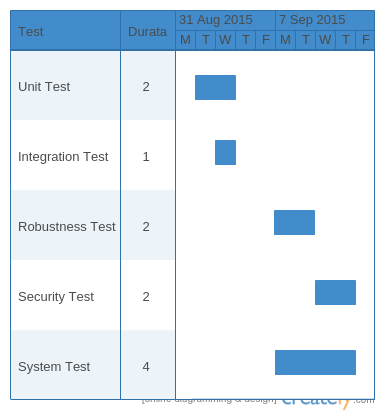
\includegraphics[trim={0 0.5cm 0 0}, clip, scale=0.5]{../TestPlan/test.png}
\end{frame}

\begin{frame}
\frametitle{Documento TestPlan: cosa?}
\small{
Divideremo i test in due grandi famiglie
\begin{itemize}	
\item White Box (test Strutturali):
\begin{itemize}	
\footnotesize{
\item Unit Test: Test sul corretto funzionamento delle classi responsabili del controllo della velocità  rispetto al limite impostato ed eventuale soglia di superamento di quest'ultimo.
\item Integration Test: Si è testata l'integrazione tra i vari componenti del sistema TMC: il simulatore SW (Modulo HW), la web application (pagine jsp), le Servlet e il DB.
\item System Test: I test in questa sezione ci hanno permesso di controllare alcune proprietà  del nostro sistema.}
\begin{itemize}	
\scriptsize{
\item Robustness Test:
Verifica dei campi in caso di anomalie (es. mail mancante o campi errati) ed eventuali risposte d'errore.
\item Security Test: Controllo sessione, Controllo permessi e autorizzazioni pagine.}
\end{itemize}
\end{itemize}
\item Black Box (test Funzionali).
\begin{itemize}	
\item Funzioni Amministratore;
\item Funzioni Utente.
\item Funzioni comuni.
\end{itemize}
\end{itemize}}
\end{frame}

\end{document}